\chapter{The Standard Model of Particle Physics}\label{chapt:SM}

This chapter is an introduction to the Elementary Particle Physics in the view of Standard Model.
First the particles are described, then the way they interract is shown. The short introduction
to the top physics is given in the end.

\section{Introduction. Elementary Particle physics}

The main question which the elementary particle physics addresses is '\textit{What is the matter made of?}'
This question was stated many thouthands years ago and is still of current interest. First guesses about
the structure of matter were made already in ancient Greece by a phylosopher-atomist Demokrit, who
claimed that everything around us consists of tiny undevidable chuncs called \textit{atomos}\cite{yangcn}.
But the elementary particle physics (elementary here means unstructured) in modern sense started with 
J.J. Thomson's discovery of \textit{electron}\cite{jjthome} in 1897. The electrons were correctly surmised to be constituents
of atoms. The full picture of the atom structure was created after Ernest Rutherford's scattering experiment\cite{rutherford},
thus proving atom to be non-elementary particle. It actually consists of a heavy positively charged core, called 
\textit{nucleus} and very light negatively charged electrons, moving around like satelites. 
The nucleus was also proven to be non-elementary. But no structure of electron was discovered 
and it is nowadays known as one of the undevidable particles. 

Many other elementary particles were subsequently discovered the last sixty years. Now having an idea 
what are the structureless bricks making up matter in the Universe, particle physycs
states another important question: '\textit{How do the particles interact?}'.

The Standard Model of particle physics is a theory which is summing up the constituents of the Universe
and interactions between them. This theory is overall successfully describing many phenomena and 
agrees with the experimental efforts. But there is also a number of challenges which Standard Model
is facing. In particular
\begin{itemize}
 \item the gravitation is not described,
 \item the neutrino oscillations and their non-zero masses are not explained,
 \item dark matter and dark energy do not fit into the model,
 \item the matter-antimatter asymmetry in the Universe is not explained.
\end{itemize}


\section{Elementary Particles}

This section gives an answer which the Standard Model gives to the question '\textit{What is the matter made of?}'.
The Standard Model asserts that all the material in the Universe is made up of the elementary \textit{fermions} (particles
which have half-integer spin -- $\frac{n}{2}\hbar$, $n = 1, 2, 3, ...$) interacting through the fields, carried 
by \textit{bosons} (particles which have integer spin -- $n\hbar$, $n = 0, 1, 2, 3, ...$). The names of the particles 
originate from the statistics they obay. Fermions follow the Fermi-Dirac statistics, bosons -- Bose-Einstein statistics.
Another thing which is different for the fermions and bosons is how their wave functions behave. After swapping two
bosons in a system, the wave function does not change, it is symmetric to the exchange of bosons. While the wave function
of fermions changes the sign, it is asymmetric.

The Fig.\ref{fig:SM_Particles} shows all the elementary constituents of matter and fields.
\begin{figure}[t]
  \centering
  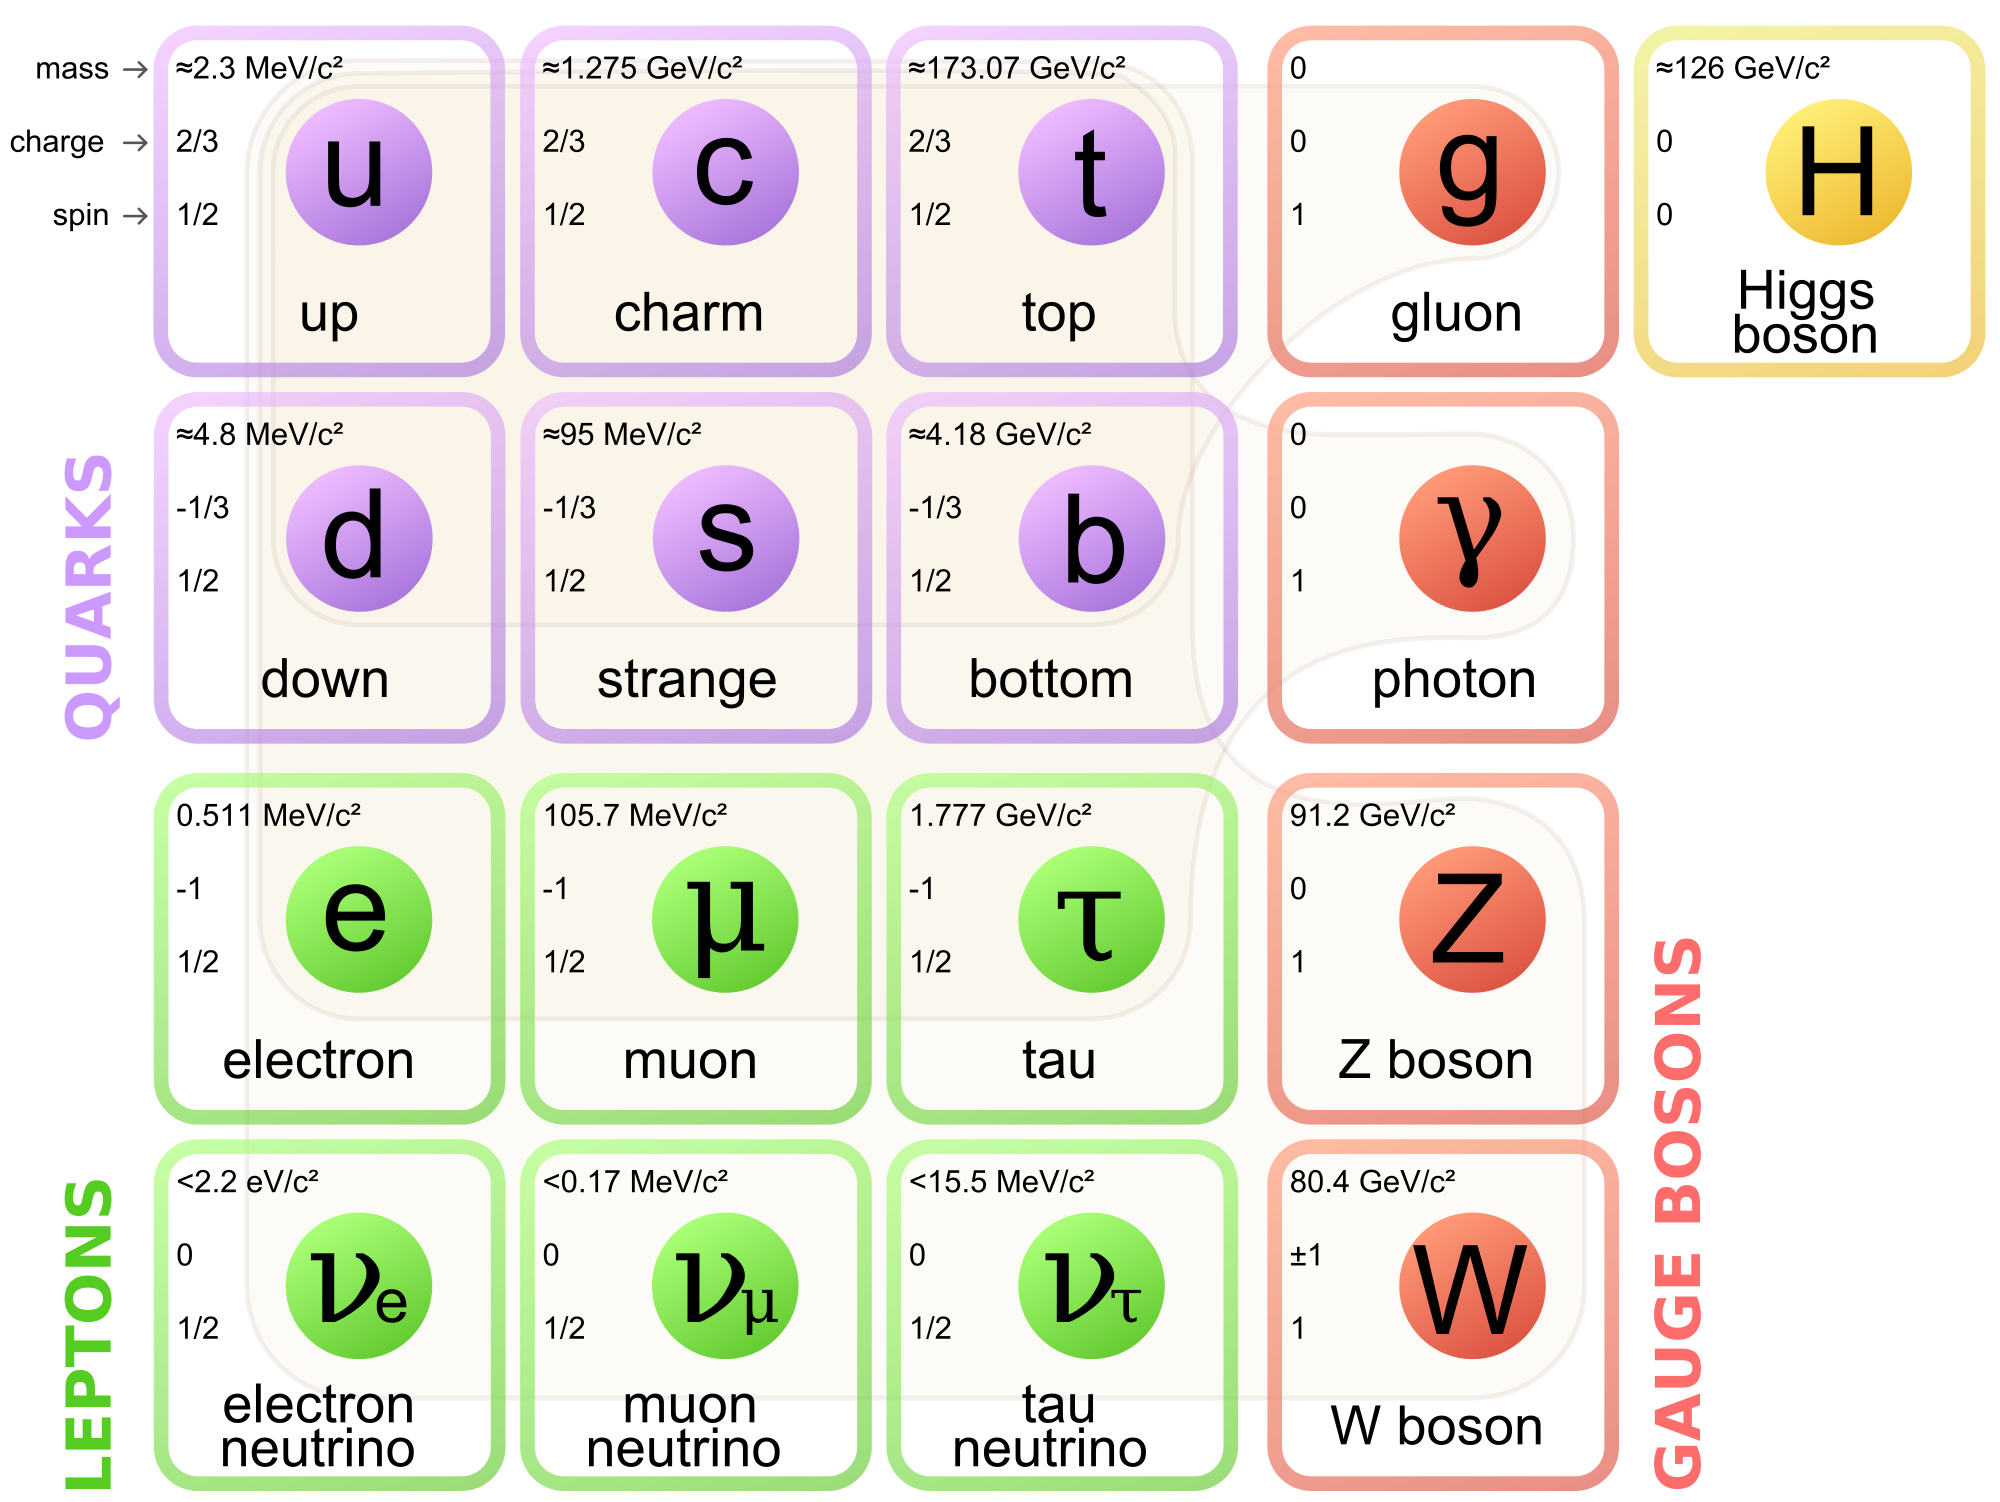
\includegraphics[width=0.6\textwidth]{01_Theory_SM/plots/Standard_Model_of_Elementary_Particles.png}
  \caption{The Standard Model of Elementary Particle Physics with three generations of matter fermions, field bosons and a Higgs boson. 
  The properties of the particles are also shown in each box.}
  \label{fig:SM_Particles}
\end{figure}


\subsection{Leptons}

The two bottom rows of fermions in the Fig.\ref{fig:SM_Particles} represent the known \textit{leptons} with their masses, charges
and spins. 

In general, the fermions are described with the Dirac equation\cite{diraceq}:

\begin{equation}\label{eq:dirac}
  i\hbar\gamma^{\mu}\partial_{\mu}\psi - mc\psi = 0 ,
\end{equation}

where the $\psi$ is a four-element Dirac spinor, an equivalent of a one dimentional Schr\"{o}dinger wave function, 
$\gamma^{\mu}$s are the gamma matricies and $\partial_{\mu}$ is a partial derivative with respect to the time-space four-vector
components. 

Dirac equation \ref{eq:dirac} has solutions with positive but also with negative energy states. Those are treated
as \textit{antiparticles}. So every lepton, being a fermion, has an antiparticle. At the Fig.\ref{fig:SM_Particles}
only particles are shown. Electron $e^{-}$ has an antiparticle positron $e^{+}$. The muon $\mu^{-}$, tau $\tau^{-}$ and
their antiparticles, $\mu^{+}$ and $\tau^{+}$ differ from the electron and positron only by their masses and their lifetimes.

Neutral leptons, neutrinos $\nu$, also have antiparticles, antineutrinos $\bar{\nu}$. Every massive lepton has a corresponding
neutrino: $\nu_{e}$, $\nu_{\mu}$ and $\nu_{\tau}$. It is believed that in the interactions a lepton can change only to another
of this type. This is known as \textit{conservation of lepton number}. In this rule leptons have positive lepton numbers and
antileptons -- negative ones.

\subsection{Quarks}\label{sec:quark}

The two upper rows in the Fig.\ref{fig:SM_Particles} list the known \textit{quarks}, showing their masses, charges and spins.

Quarks, being fermions, are also described by the Dirac equation. However, there is a number of properties which are very different
to the leptons. They have non-integer electric charge ($\frac{2}{3} e$ or $-\frac{1}{3} e$, where $e$ is the electron charge) and a 
\textit{flavour} (up, down, charm, strange, top and bottom).

Quarks have another charge called \textit{color}. All the observed isolated objects can't have color, they are colorless. Thus, the 
quarks have never been observed in isolated state. The system of quarks are called \textit{hadrons}. The most elementary hadrons are 
\textit{baryons}, which consist of three quarks, and \textit{mesons}, which consist of two quarks. The only stable yet known baryon 
is the proton. All the mesons are unstable.

The barions are fermions as they consist of an odd number of quarks which have half an iteger spins. Thus, the mesons have integer spins
(0 or 1). This means that mesons are bosons.

\section{Interactions}

An interaction is the way how particles show and organize themselves in the environment. The interaction is performed through exchange
of the mediator bosons.

Nowadays only four basic interactions are known: \textit{strong}, \textit{electromagnetic}, \textit{weak} and \textit{gravitational}. 
Each of them can be characterized with a \textit{strength} $Fr^2$, where $F$ is the force and $r^2$ is the squared distance between two interacting objects.
The following table shows the rough order of the interaction strengths\footnote{The strength of the interaction depends on the nature of the 
interacting objects. That is why the values in the table should be concerned as the measure of order, not an exact number.}, the mediator
and the theory, which describes these interactions \cite{griffiths2008introduction}:

\begin{center}\label{tab:forces}
  \begin{tabular}{ | c | c | c | c | }
    \hline
    \textbf{Interaction} & \textbf{Strength} & \textbf{Theory} & \textbf{Mediator} \\ \hline \hline
    Strong & 10 & Quantum Chromodynamics & Gluon \\ \hline 
    Electromagnetic & 10$^{-2}$ & Quantum Electrodynamics & Photon \\ \hline
    Weak & 10$^{-13}$ & Flavordynamics & $W$ and $Z$ Bosons \\ \hline
    Gravitation & 10$^{-42}$ & Geometrodynamics & Graviton \\
    \hline
  \end{tabular}
\end{center}

More details on every interaction is presented in this section.

\subsection{Electrmagnetic Interaction}

The theory behind the electromagnetic interactions -- quantum electrodynamics (QED) -- was developed earlier than other interactions theories
and is the most successful one. It describes the interactions between the elementary electrically charged fermions via mediator photons.
The electromagnetic interaction is such that the oppositely electrically charged objects attract each other while the same sign charges repulse.
This interaction is present on any distance getting weaker proportionally to the distance squared. The QED is based on the gauge group $U(1)$.
Every electromagnetic phenomena is ultimately reducible to the following elementary process:

\begin{figure}[h]
  \centering
  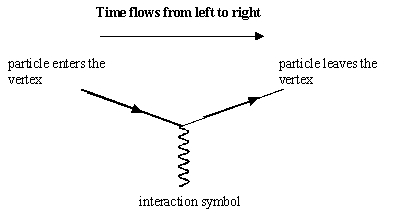
\includegraphics[width=0.6\textwidth]{01_Theory_SM/plots/QED_simple.png}
  \caption{Feynman graph of the elementary QED process.}
  \label{fig:QED_simple}
\end{figure}

The more complex processes can be described combining two or more of these elementary verteces.

A coupling constant, or the interaction strength of the electromagnetic interaction is given as following:

\begin{equation}
 \alpha = \frac{e^{2}}{4\pi\epsilon_{0}\hbar c} \approx \frac{1}{137},
\end{equation}

where $\epsilon_{0}$ is the permitivity of vacuum, $e$ is the electron charge and $c$ is the speed of light.

As coupling constant is small ($\alpha \ll 1$), it can be used for the expansion in the perturbative calculations.
Each term of this expansion will have a term of $\alpha$. Thus, the naming of the processes lying beyond each of the term
is Leading Order process (LO), Next-to-Leading Order process (NLO), Next-to-Next-to-Leading Order process (NNLO), etc.

\subsection{Strong Interaction}

The theory which describes the strong interaction is the Quantum Chromodynamics (QCD), which is based on the gauge group $SU(3)$. Only the
objects which have a color charge can interact strongly. The color charge (first mentioned in sec. \ref{sec:quark}) has three eigenstates:
red (r), blue (b) and green (g). As for the any other charge, the color charge eigenstates have also anticharges -- anicolors. The combination
of the color and corresponding anticolor, as well as the combination of all the colors/anticolors results the colorless state.

The mediators of the strong interaction are gluons. These particles are massless and carry two colors -- color and anticolor. Thus, the strong 
interaction is the interaction between quarks via gluons. The color charge is conserved during the interaction.

The coupling constant of the strong interaction, $\alpha_{s}$, is a running constant depending on the energy scale $Q$. As shown in the
Fig. \ref{fig:Alpha_s}, the $\alpha_{s}$ rapidly increases with the lessening of the $Q$. This means that on the larger distances 
the strength of the interaction increases a lot. This phenomenon is called \textit{confinement} and this is the reason why the quarks
can't exist in the isolated state. The more the quarks separate from each other in terms of distance, the stronger they interact, the harder
it becomes to divide them. Even if one always has enough energy to separate quarks more and more from each other, they gluon field will become critically
high and produce the quark-antiquark pair. This process may repeat sequentially. This constantly happens under the conditions created in the
particle colliders. The phenomenon of sequential quark pair production is called \textit{hadronization}.

The confinement constrains the maximum distances on which the interaction in terms of the gluon field is observed before producing the quark-antiquark pair.
The limit of the region of strong interaction impact is of the order of the nucleon size -- $\sim 10^{-15}$ m.

\begin{figure}[t]
  \centering
  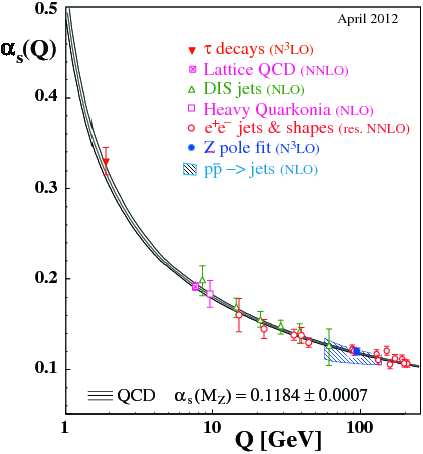
\includegraphics[width=0.6\textwidth]{01_Theory_SM/plots/Alpha_s.png}
  \caption{Summary of measurements of $\alpha_s$ as a function of the respective energy scale $Q$. The respective degree of QCD perturbation 
  theory used in the extraction of $\alpha_{s}$ is indicated in brackets (NLO: next-to-leading order; NNLO: next-to-next-to leading order; 
  res. NNLO: NNLO matched with resummed next-to-leading logs; N3LO: next-to-NNLO). Figure taken from \cite{PDG-2012}.}
  \label{fig:Alpha_s}
\end{figure}

The opposite tendency which can be observed in Fig. \ref{fig:Alpha_s} is that the $\alpha_{s}$ is getting smaller for the higher values 
of the $Q$. This means that for the shorter interaction distances, the coupling constant becomes weaker. This phenomenon carries the 
name \textit{asymptotic freedom}. Under these conditions the quarks are assumed to be treated as the free particles. The asymptotically 
free quarks are assumed to be observed in the \textit{quark-gluon plasma} \cite{Bohr1977275} -- the state of matter with extremely high density and/or temperature.

The conjectured QCD states, depending on temperature and density, are shown in Fig. \ref{fig:QGP}.

\begin{figure}[t]
  \centering
  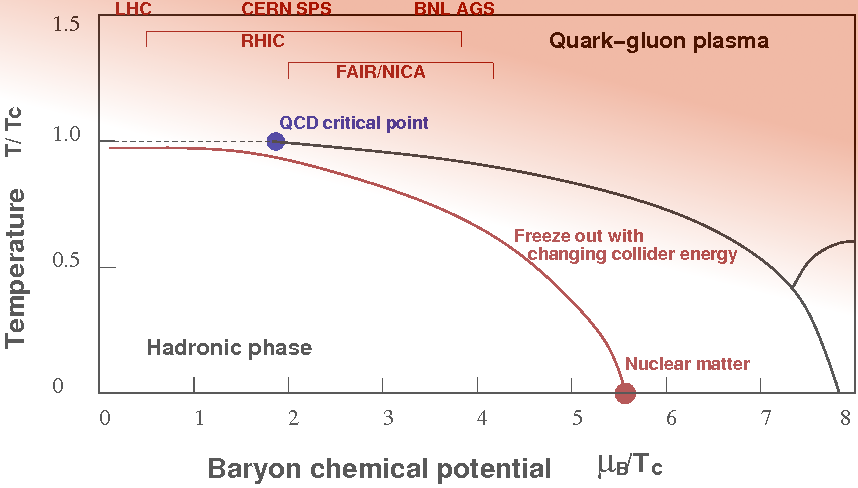
\includegraphics[width=0.8\textwidth]{01_Theory_SM/plots/QGP.png}
  \caption{Conjectured phase diagram of QCD. The different states and phase curves are shown. The energy and density range of different high energy 
  physics experiments are marked on the top of the figure.}
  \label{fig:QGP}
\end{figure}

\subsection{Weak Interaction}

As it can be seen in the table \ref{tab:forces}, the strength of the weak interaction is many orders of the magnitude smaller than the once for the 
electromagnetic and strong interaction. This fact explains the name \textit{weak}.

The weak interaction differs from the others in a way that there is no particular name for the charge responsible for this interaction 
(like electrical charge for the electromagnetism and color charge for the strong interaction). All the leptons and quarks carry the ability to interact
weakly. A widely known example of the weak interaction is the process of the $\beta$-decay.

There are 

% \subsection{Weak Interaction and Electroweak Symmetry Breaking}
% \subsection{Gravitation}
% 
% \section{Top Physics}
% \subsection{Top Quark Production}
% \subsection{Top Quark Decay}
